\chapter{Colocalization}\label{ch:colocalization}

When creating a point in the Unreal Engine instance on the handheld device then it's coordinates are considered in reference to the world coordinate system of the Unreal Engine game. In order for the excavator to be able to use the set geometric location it has to be converted into a representation with respect to the excavator's coordinate system.

As previously mentioned the approach used in this work was to extract Azure Spatial Anchors from the excavator's camera view using a ROS wrapper and after uploading them to Azure Cloud retrieve them using an Unreal Engine plugin on the mobile device. In the end this allows us to find the relative transformation from the UE world coordinate origin to the excavator's coordinate origin which is represented by the pose of the detected anchor.

\section{Azure Spatial Anchors}\label{sec:azure_spatial_anchors}

An Azure Spatial Anchor works in the following way: 
\begin{itemize}
    \item By scanning the environment visual reference points are detected.
    \item When enough visual information is received the initial pose of the scan can be stored by creating an anchor at that position.
    \item This anchor can then be uploaded to the Azure cloud to be retrieved whenever a device detects the visual surrounding encoded in the anchor.
    \item Note: When scanning the environment an anchor can also be placed at a set location with respect to the origin as opposed to the origin itself.
\end{itemize}

In this project the pose to track and to store in the Azure Cloud was the origin of the camera device itself. This made it possible to find the relative transformation between the coordinate systems.

The advantage of using Azure Spatial Anchors is that the colocalization is completely taken care of by creating and detecting an anchor due to the visual information of the environment that is encoded within it.

\section{Colocalization Testing}\label{sec:colocalization_testing}

For the testing of the proposed pipeline a Realsense t-265 tracking camera was used which represented the camera view from the excavator. 

Two different environments were used to perform the colocalization tests. A meadow and a mostly empty parking lot:

\begin{figure}[htp]
    \centering
    \subfloat[Meadow]{
    \includegraphics[scale = 0.09]{images/colocalization/meadow.jpg}
        \label{fig:meadow}
        }
        \hfill
    \subfloat[Parking Lot]{
        \includegraphics[scale = 0.09]{images/colocalization/parking_lot.jpg}
        \label{fig:parking_lot}
        }
        \hfill
    \caption{Testing Environments}
    \label{fig:environments}
\end{figure}

For the following tests the setup was always the same:
\begin{itemize}
    \item The t-265 camera was started at a prominent point and the environment was scanned.
    \item An anchor was created (supposedly at the starting position) using the visual information registered.
    \item The handheld UE app was started at a random position spawning an AR excavator model at that pose.
    \item The anchor was detected by the handheld UE instance and using the relative transform the excavator model was shifted to that pose.
\end{itemize}

\subsection{Testing: Meadow Environment}\label{subsec:meadow}


\begin{figure}[ht]
    \centering
    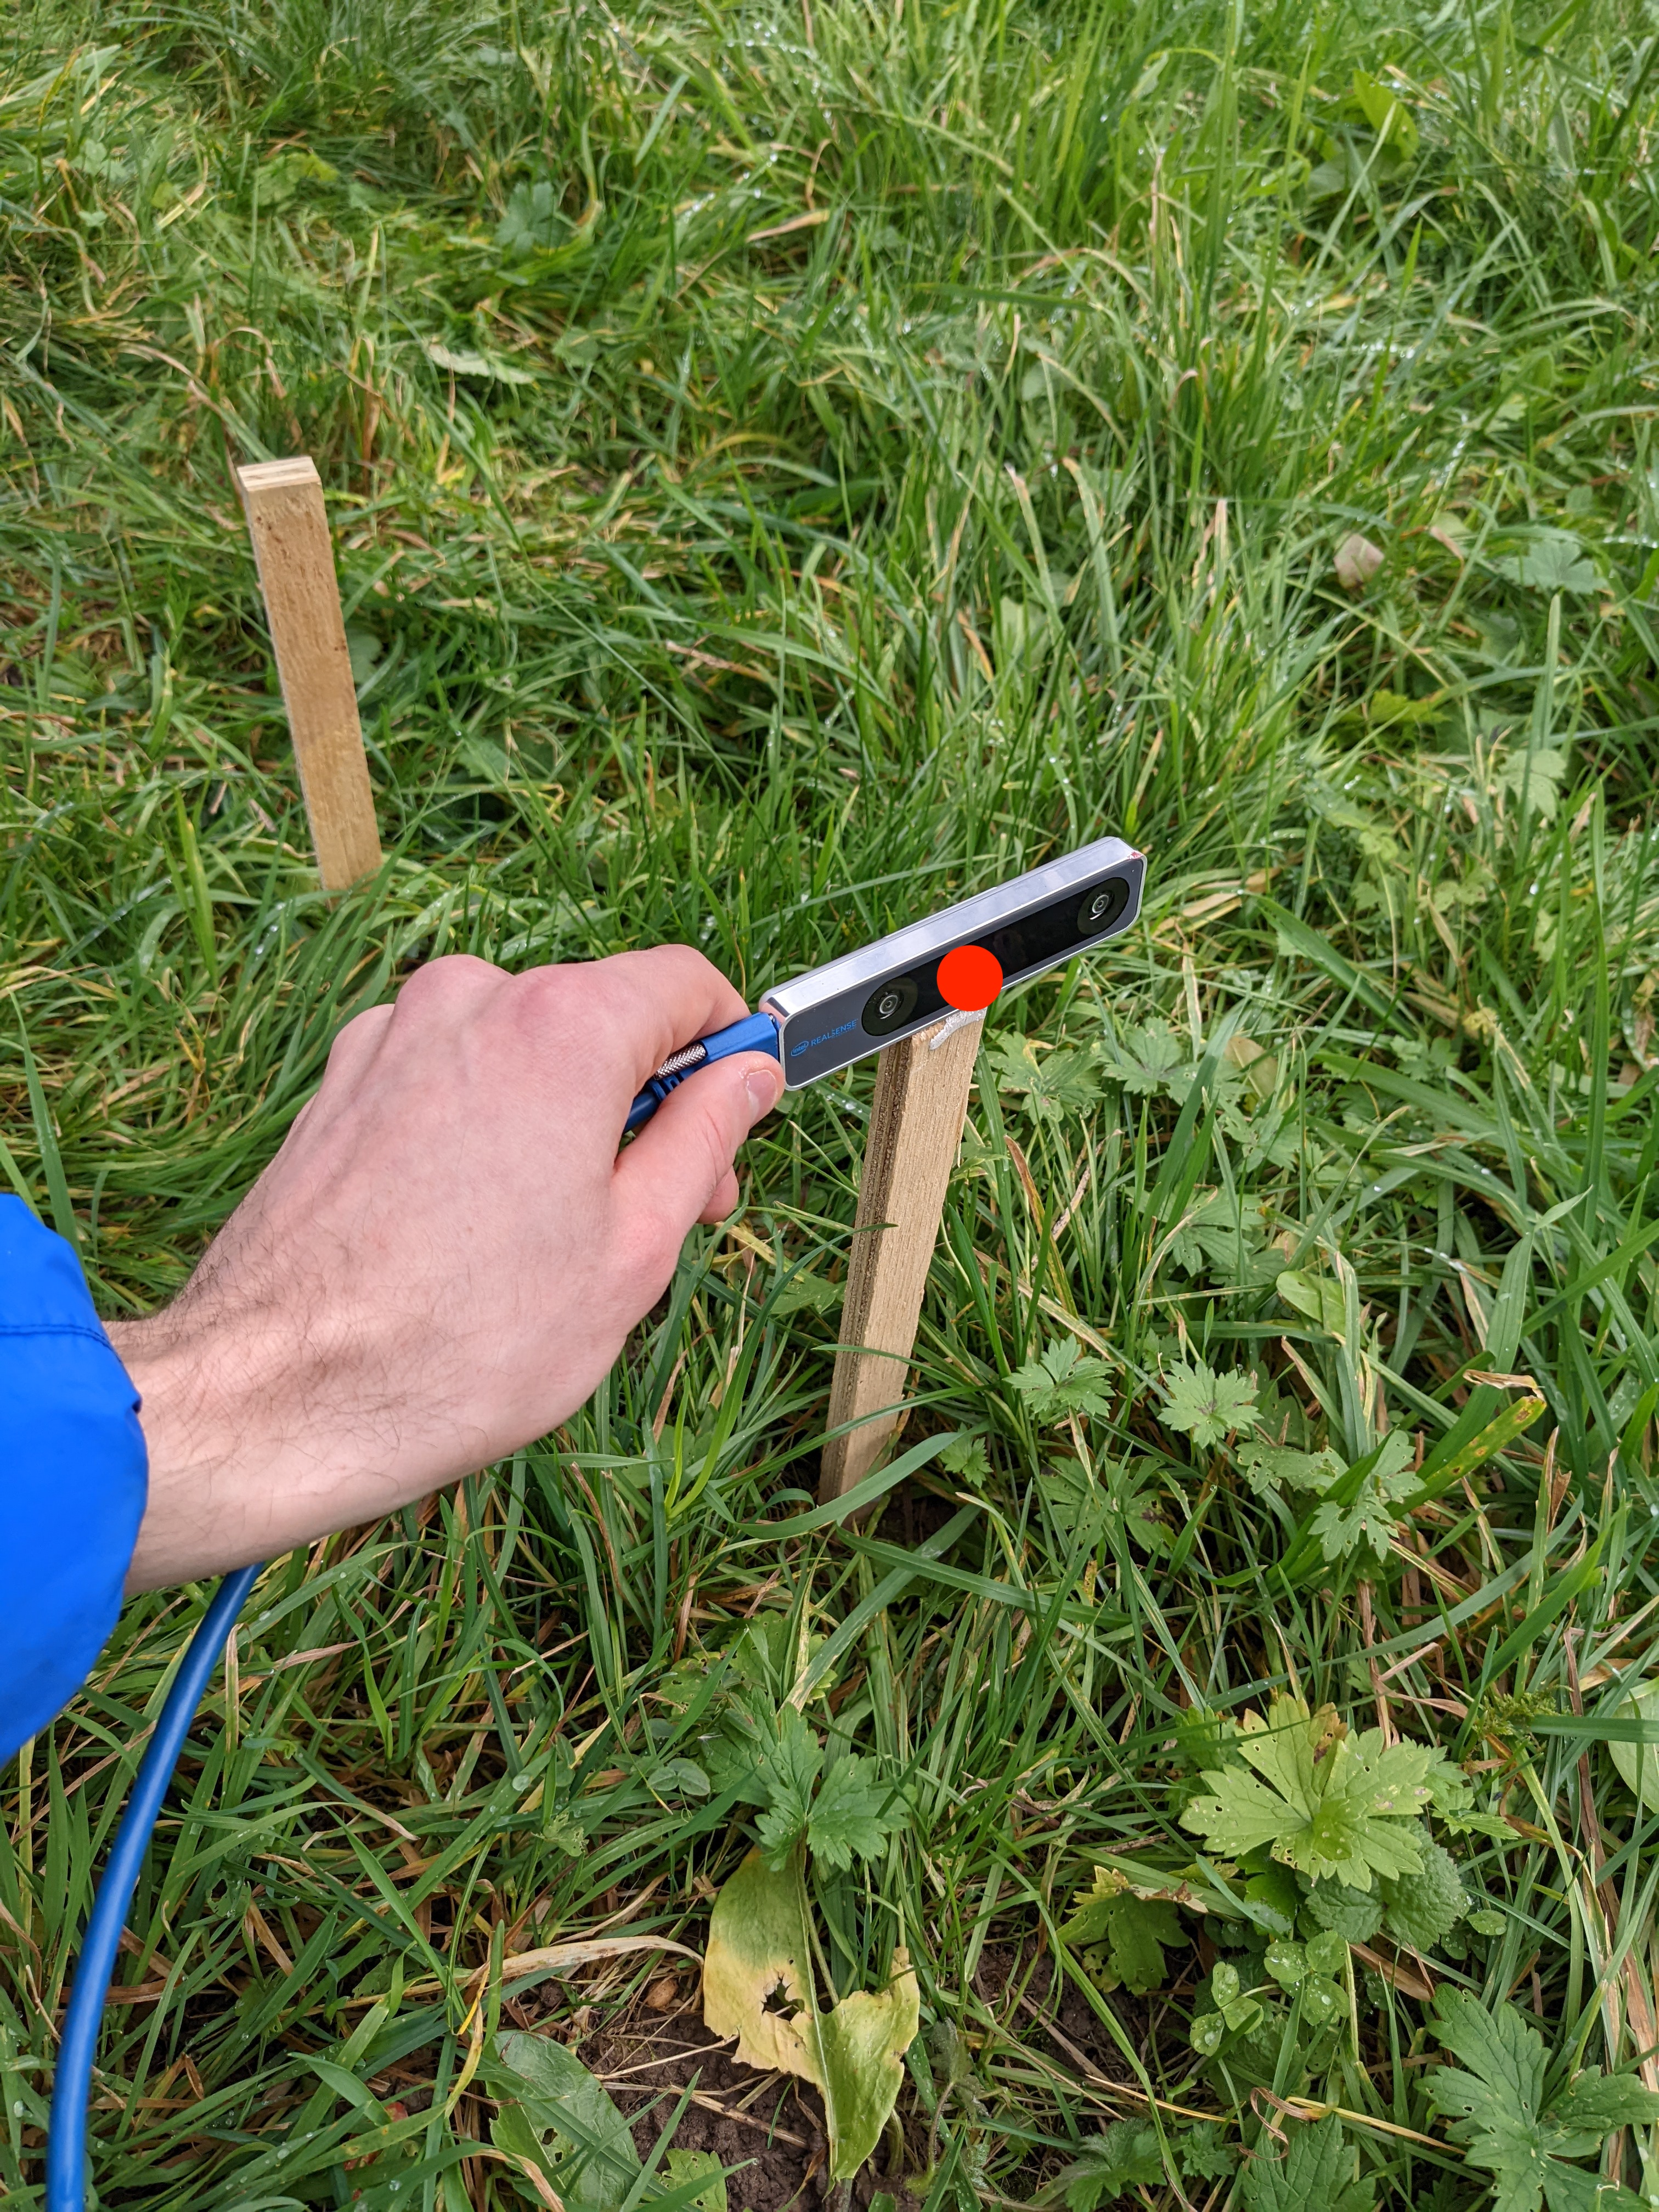
\includegraphics[scale = 0.1]{images/colocalization/meadow_start.jpg}
    \label{fig:meadow_start}
    \caption{Camera origin representing the location where to place an anchor}
\end{figure}
\clearpage

\begin{figure}[htp]
    \centering
    \subfloat[Excavator pose at initialized UE world origin]{
        \includegraphics[scale = 0.165, trim={6cm 0 1cm 0}, clip]{images/colocalization/meadow_before.png}
        \label{fig:meadow_before}
        }
        \hfill
    \subfloat[Excavator pose after colocalization]{
        \includegraphics[scale = 0.165, trim={6cm 0 1cm 0}, clip]{images/colocalization/meadow_after.png}
        \label{fig:meadow_after}
        }
        \hfill
    \caption{Meadow Colocalization}
    \label{fig:meadow_basic}
\end{figure}

As can be seen in \cref{fig:meadow_basic} after the colocalization the excavator together with the world origin is relocated to a new pose. There is however a shift between the supposed anchor location (indicated with an afterwards inserted red dot) and the new location the excavator assumes. This can be traced back to a shift in the anchor creation. 

\clearpage

\subsection{Testing: Parking Lot Environment}\label{subsec:parking_lot}

\begin{figure}[ht]
    \centering
    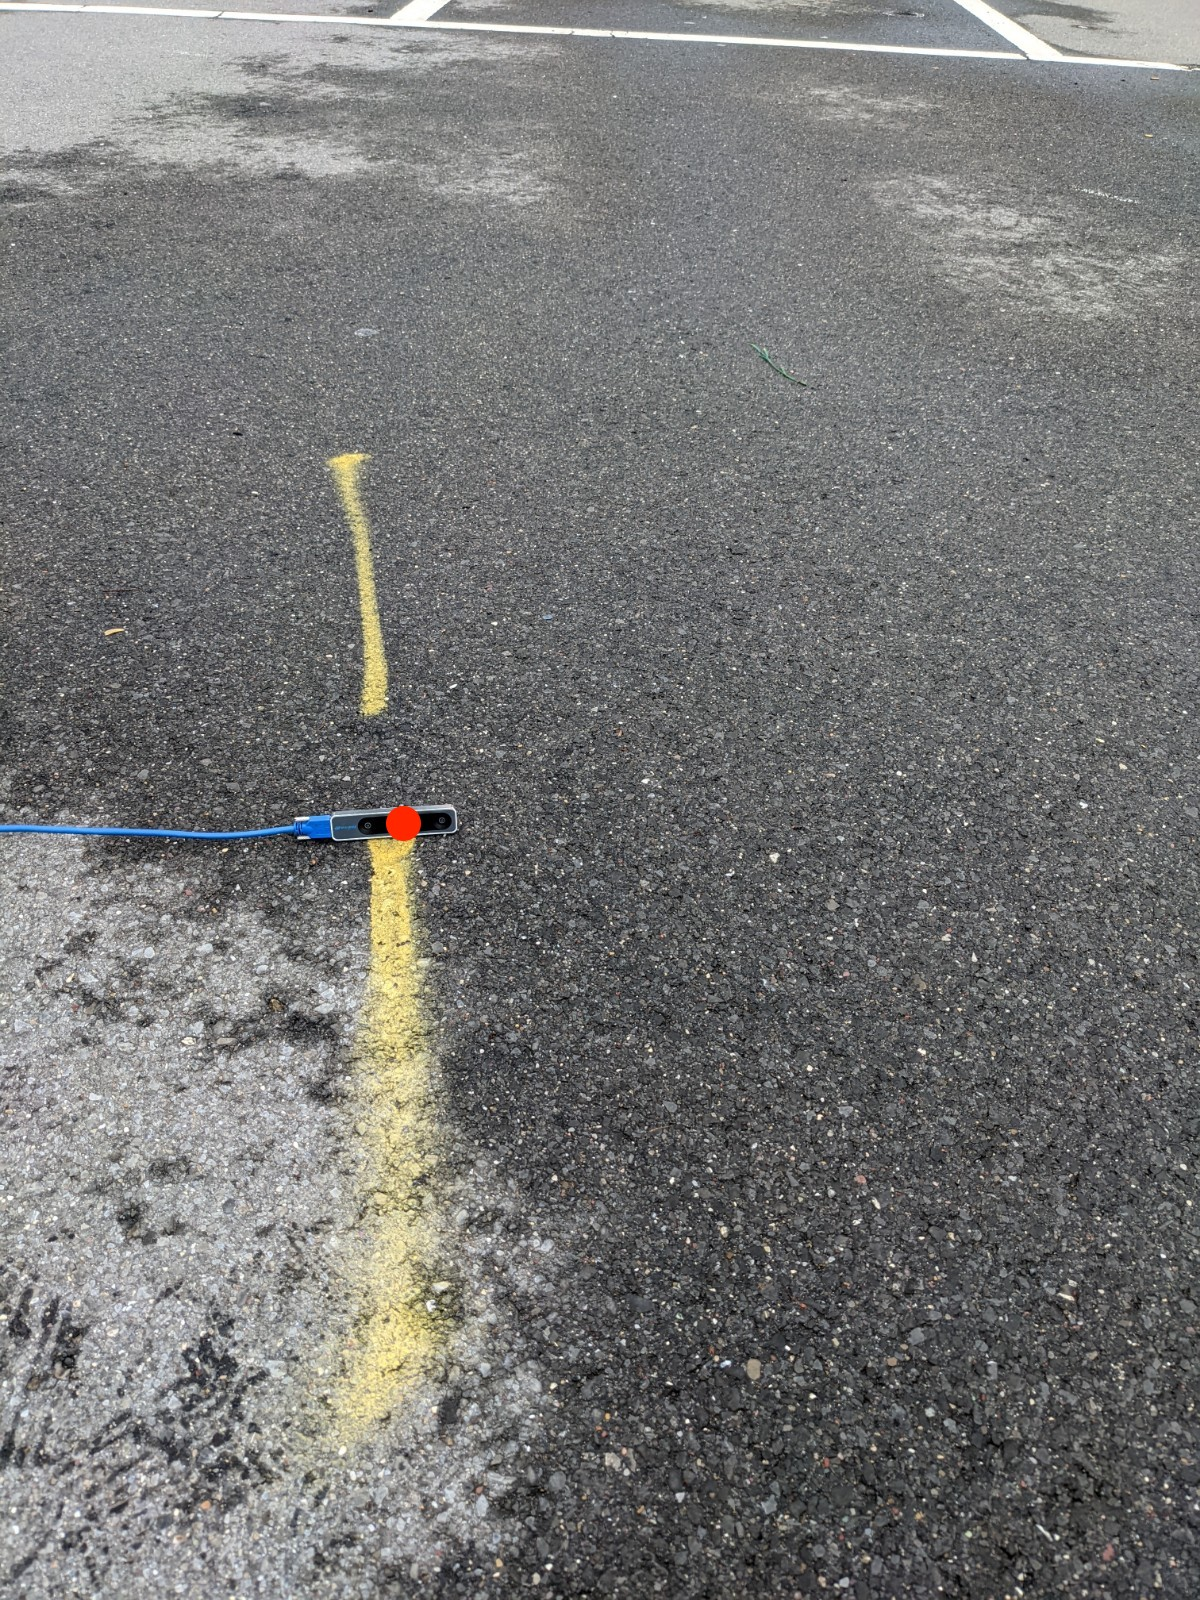
\includegraphics[scale = 0.28]{images/colocalization/parking_lot_start.jpg}
    \label{fig:parking_lot_start}
    \caption{Camera origin representing the location where to place an anchor}
\end{figure}
\clearpage

\begin{figure}[htp]
    \centering
    \subfloat[Excavator pose at initialized UE world origin]{
        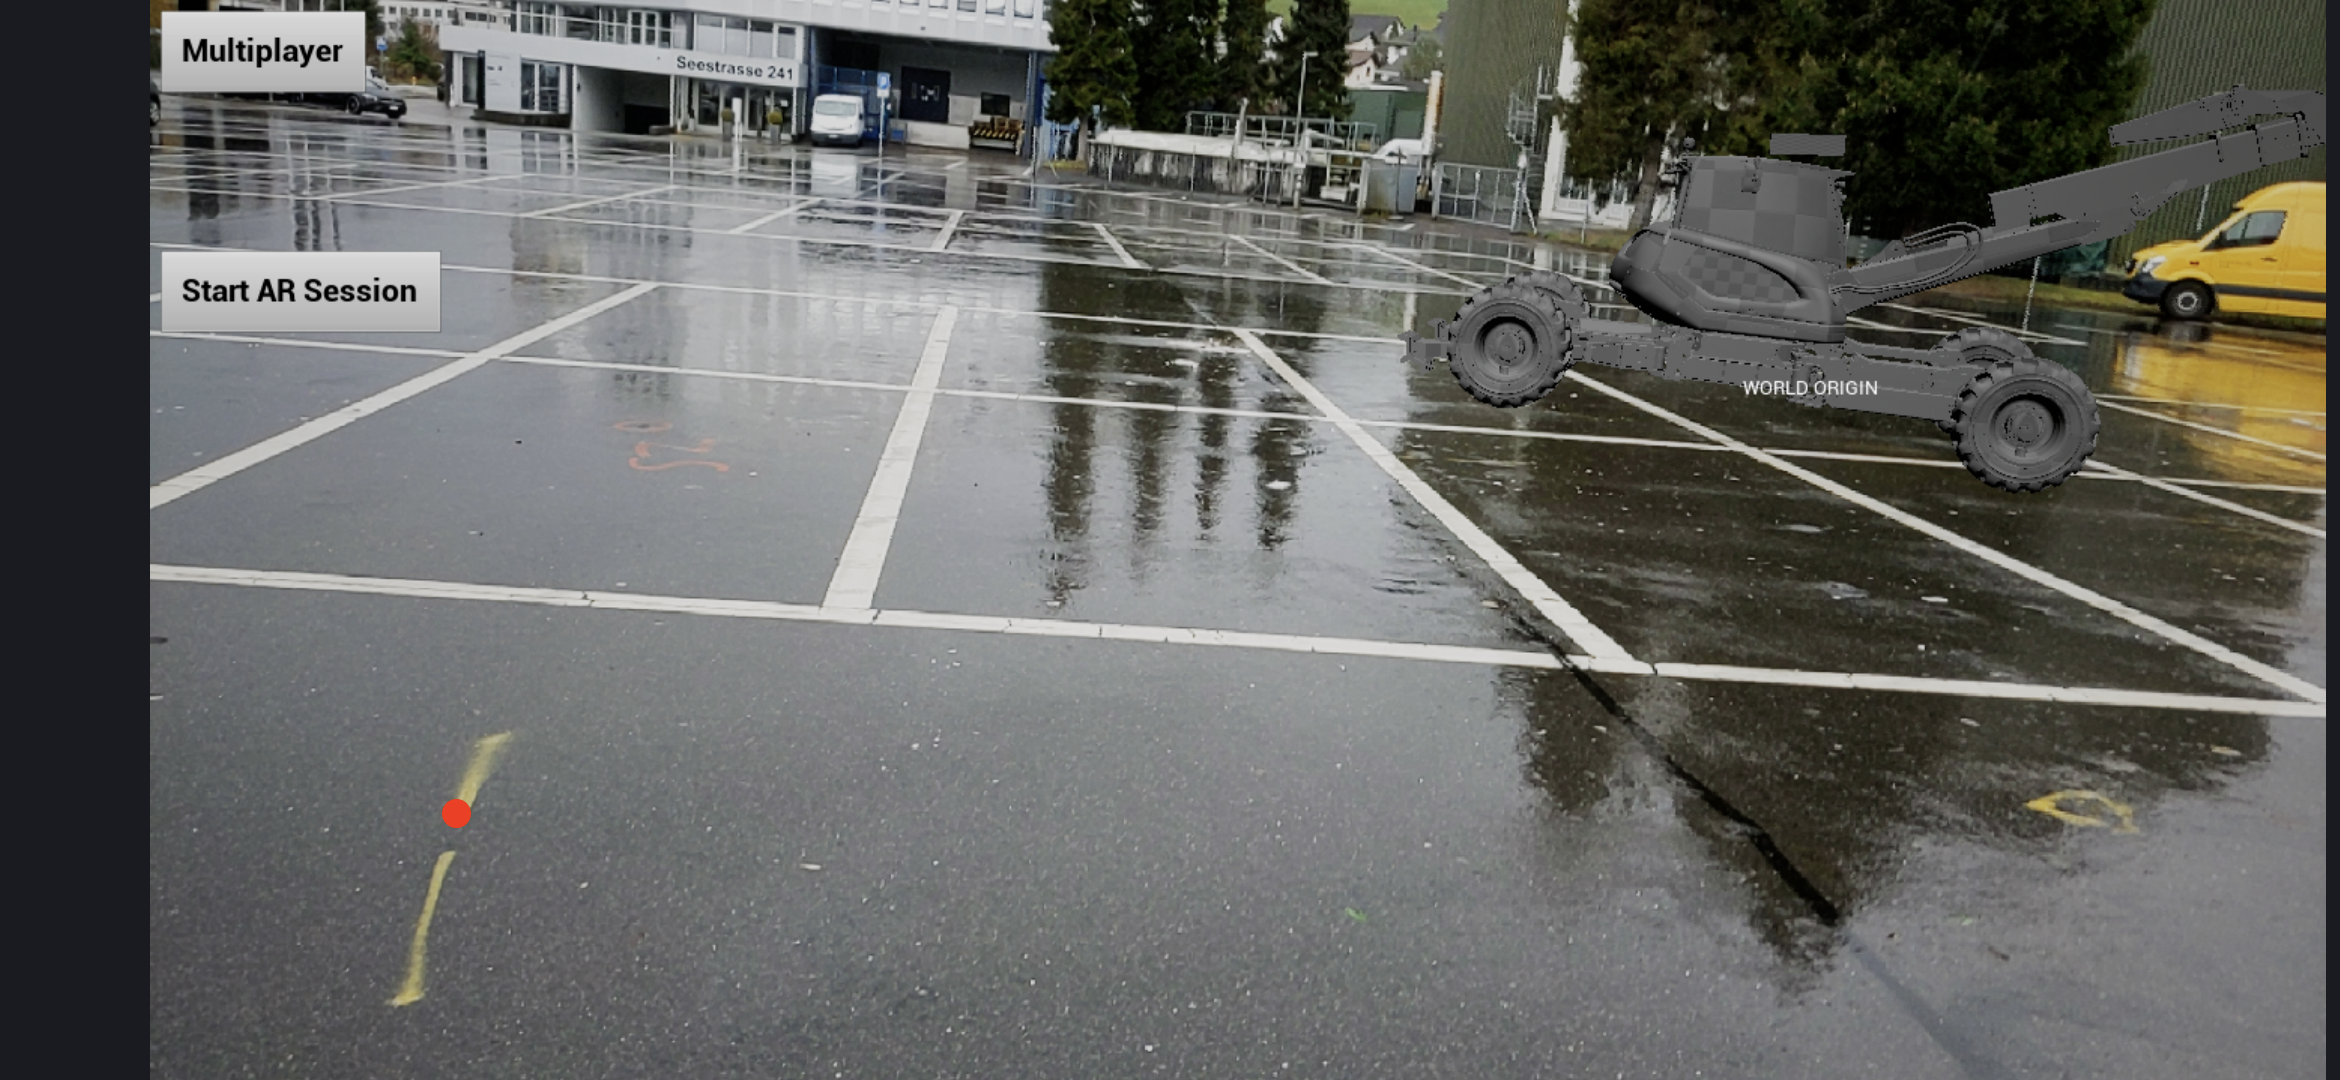
\includegraphics[scale = 0.165, trim={6cm 0 1cm 0}, clip]{images/colocalization/parking_lot_before.png}
        \label{fig:parking_lot_before}
        }
        \hfill
    \subfloat[Excavator pose after colocalization]{
        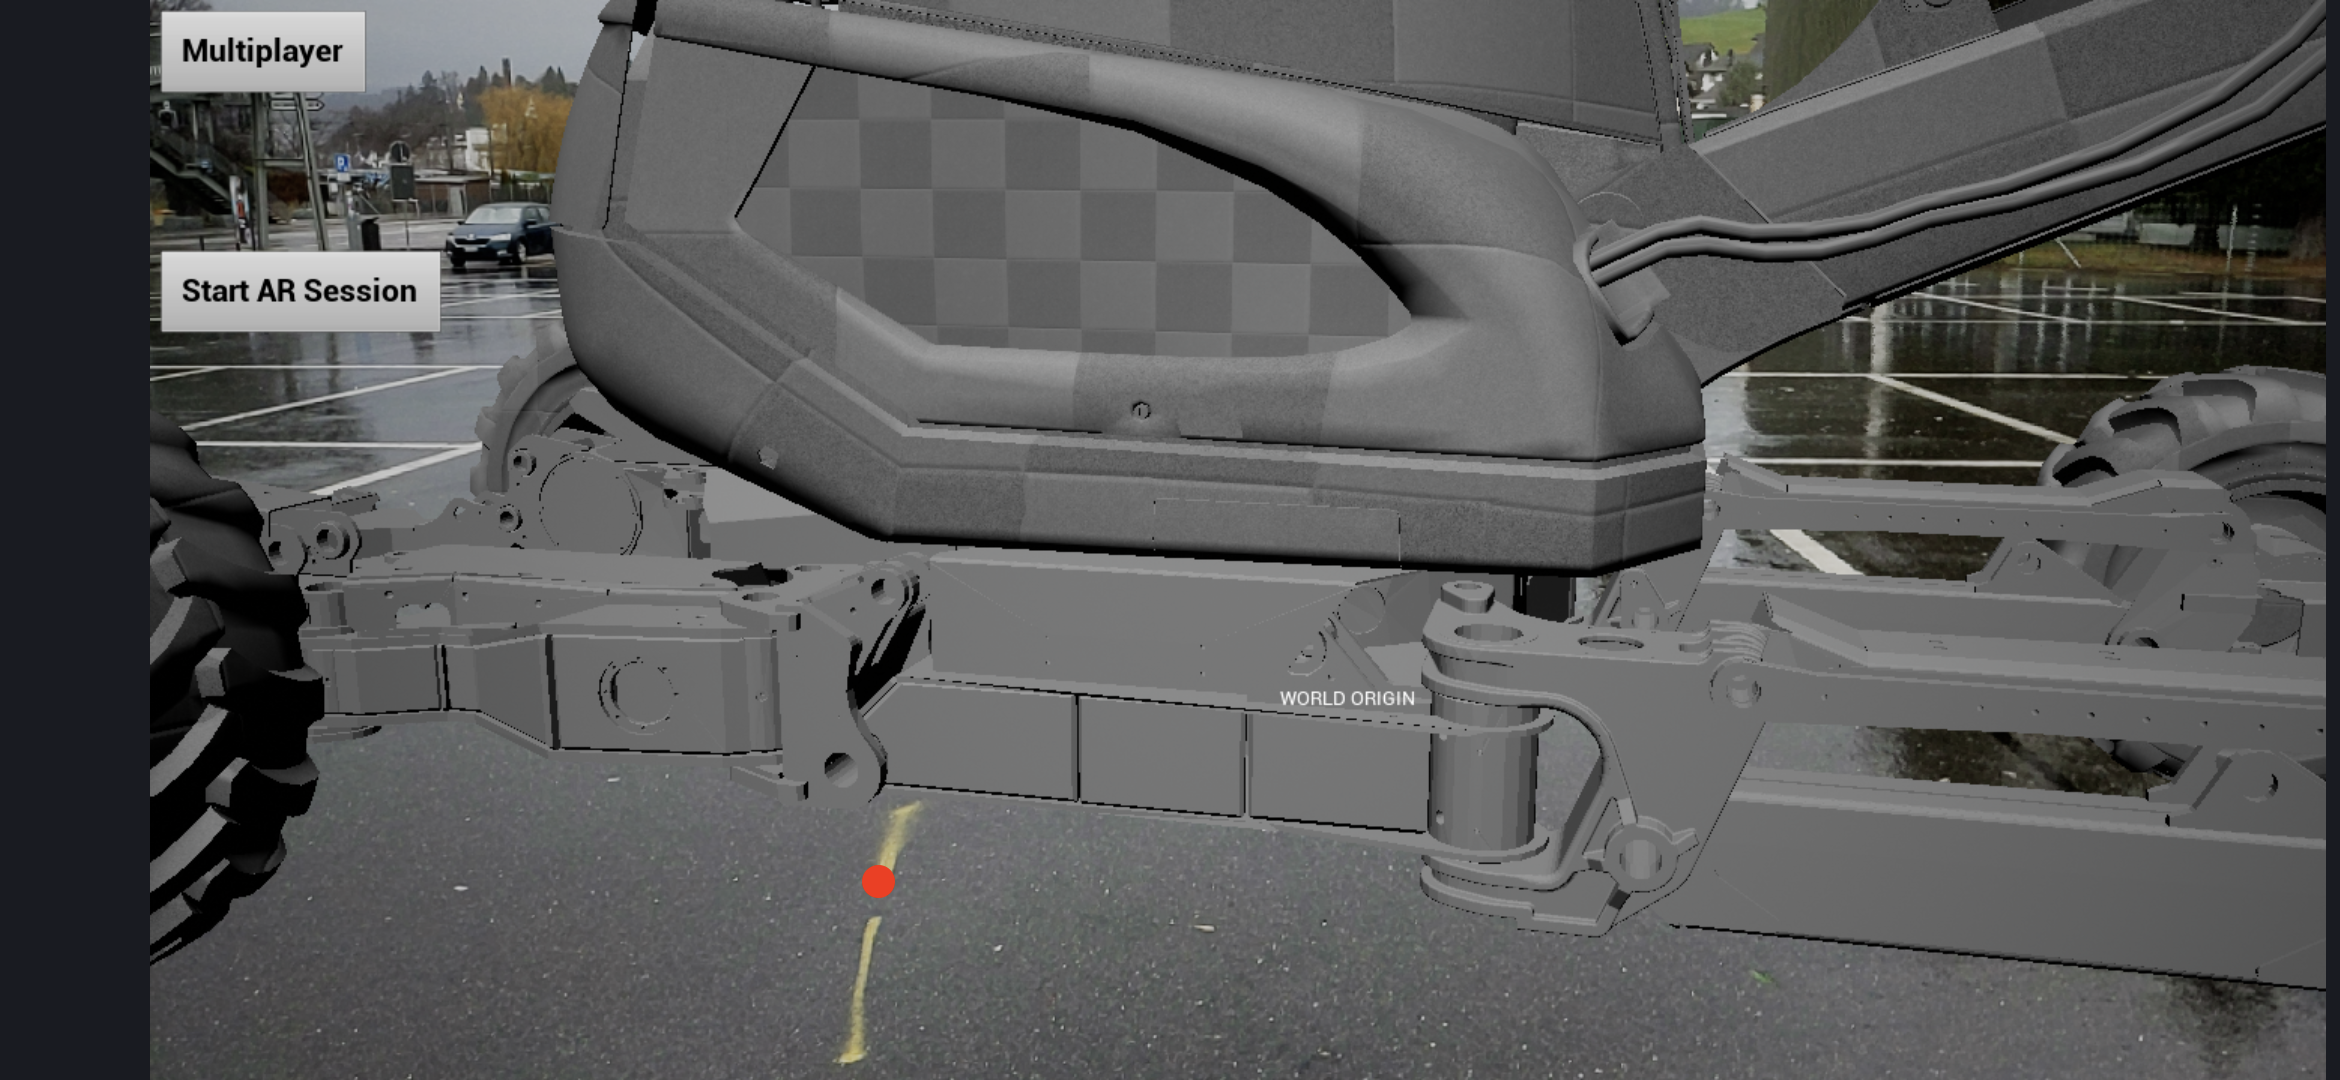
\includegraphics[scale = 0.165, trim={6cm 0 1cm 0}, clip]{images/colocalization/parking_lot_after.png}
        \label{fig:parking_lot_after}
        }
        \hfill
    \caption{Parking Lot Colocalization}
    \label{fig:parking_lot_basic}
\end{figure}

Here we have a similar performance as with the meadow environment. A "correct" relocalization to a shifted initial anchor. 

\subsection{Robustness}\label{subsec:robustness}

When doing the same test with different ambient circumstances like variations in lighting or weather we can see quite robust results. For instance the anchor point for the parking lot environment was created at a somewhat dry period of the day while the anchors were detected when the ground was really wet. Looking at \cref{subsec:ambient} we can also see robust results for worse lighting conditions in the evening.

The second kind of robustness that was tested in this setup was the repeatability of this process from different starting poses of the handheld device. The results thereof can be seen in \cref{subsec:repeatability}. The same conclusion can be drawn yet again: we have a very consistent behavior considering the fact that the anchor created is off.

\subsection{Testing Conclusion}\label{subsec:testing_conclusion}

We find that we have a persisting error when creating the visual anchors with the t-265 Tracked Camera. Given these shifted anchors however the colocalization process is very accurate and robust regarding changes in illumination, weather and starting handheld position.

Also the different environments didn't seem to have a significant influence on the colocalization performance.

\section{Alternative Location Sharing}\label{sec:alternative_location_transfer}

Taking a step back the initial reason to establish colocalization was to send a high level spatial input from the handheld device to the excavator.

Note that the transmission of any location in the form of a spatial anchor could work. In the case of the origin being transmitted we get a transformation between the coordinate systems which can be used for any further point created in the handheld UE. However, only as long as the excavator does not move. 

An alternative possibility to send a touch location from the handheld input to the excavator and receive it in that frame of reference would be to use Azure Spatial Anchors directly. In that case a point would be created in UE using the intersection of the touch input's virtual line and the first obstacle hit (usual touch input point generation). Instead of transmitting this points location in the world coordinate system through UE, an anchor would be created encoding that location and sent up to the Cloud. It would be using the same Azure Spatial Anchor connection as before but in the other direction. An advantage from this approach would be that there is no dependence on a correct and persistent transformation to the excavator position. At any given time an anchor could be created and transferred without worrying about the relative transformation between the two systems.